% Communication with make =============================================

\def\GRAPHPATH{localgraphics}

\ifdefined\HANDOUT
  \documentclass[handout,aspectratio=1610,dvipsnames]{beamer}
  \def\GRAPHPATH{graphics}
\else
  \documentclass[aspectratio=1610,dvipsnames]{beamer}
\fi

\ifdefined\TITLE
\else
  \def\TITLE{}
\fi

\usepackage[ngerman]{babel}
\usepackage{ifthen}
\usepackage{color}
\usepackage{colortbl}
\usepackage{textcomp}
\usepackage{multirow}
\usepackage{nicefrac}
\usepackage{multicol}
\usepackage{langsci-gb4e}
\usepackage{verbatim}
\usepackage{cancel}
\usepackage{graphicx}
\usepackage{hyperref}
\usepackage{verbatim}
\usepackage{boxedminipage}
\usepackage{adjustbox}
\usepackage{rotating}
\usepackage{booktabs}
\usepackage{bbding}
\usepackage{pifont}
\usepackage{multicol}
\usepackage{stmaryrd}
\usepackage{FiraSans}
\usepackage{soul}
\usepackage{tikz}
\usepackage[linguistics]{forest}
\usepackage[maxbibnames=99,
  maxcitenames=2,
  uniquelist=false,
  backend=biber,
  doi=false,
  url=false,
  isbn=false,
  bibstyle=biblatex-sp-unified,
  citestyle=sp-authoryear-comp]{biblatex}

% Biblatex ============================================================

\addbibresource{rs.bib}

% Colors ==============================================================

\definecolor{grau}{rgb}{0.5,0.5,0.5}
\definecolor{lg}{rgb}{0.8,0.8,0.8}
\definecolor{trueblue}{rgb}{0.3,0.3,1}
\definecolor{ltb}{rgb}{0.8,0.8,1}
\definecolor{lgr}{rgb}{0.5,1,0.5}
\definecolor{orongsch}{RGB}{255,165,0}
\definecolor{gruen}{rgb}{0,0.4,0}
\definecolor{rot}{rgb}{0.7,0.2,0.0}
\definecolor{tuerkis}{RGB}{63,136,143}
\definecolor{braun}{RGB}{108,71,65}
\definecolor{blaw}{rgb}{0,0,0.9}
\newcommand{\gruen}[1]{\textcolor{gruen}{#1}}
\newcommand{\blaw}[1]{\textcolor{blaw}{#1}}
\newcommand{\rot}[1]{\textcolor{rot}{#1}}
\newcommand{\blau}[1]{\textcolor{trueblue}{#1}}
\newcommand{\orongsch}[1]{\textcolor{orongsch}{#1}}
\newcommand{\grau}[1]{\textcolor{grau}{#1}}
\newcommand{\whyte}[1]{\textcolor{white}{#1}}
\newcommand{\tuerkis}[1]{\textcolor{tuerkis}{#1}}
\newcommand{\braun}[1]{\textcolor{braun}{#1}}

% Newcommands =========================================================

\newcommand{\Dim}{\cellcolor{lg}}
\newcommand{\Dimblue}{\cellcolor{ltb}}
\newcommand{\Dimgreen}{\cellcolor{lgr}}
\newcommand{\Sub}[1]{\ensuremath{_{\text{#1}}}}
\newcommand{\Up}[1]{\ensuremath{^{\text{#1}}}}
\newcommand{\UpSub}[2]{\ensuremath{^{\text{#1}}_{\text{#2}}}}
\newcommand{\Spur}[1]{t\Sub{#1}}
\newcommand{\Ti}{\Spur{1}}
\newcommand{\Tii}{\Spur{2}}
\newcommand{\Tiii}{\Spur{3}}
\newcommand{\Tiv}{\Spur{4}}
\newcommand{\Ck}{\CheckmarkBold}
\newcommand{\Fl}{\XSolidBrush}
\newcommand{\xxx}{\hspaceThis{[}}
\newcommand{\zB}{z.\,B.\ }
\newcommand{\down}[1]{\ensuremath{\mathrm{#1}}}
\newcommand{\Zeile}{\vspace{\baselineskip}}
\newcommand{\Halbzeile}{\vspace{0.5\baselineskip}}
\newcommand{\Viertelzeile}{\vspace{0.25\baselineskip}}
\newcommand{\KTArr}[1]{\ding{226}~\textit{#1}~\ding{226}}
\newcommand{\Ast}{*}
\newcommand{\SL}{\ensuremath{\llbracket}}
\newcommand{\SR}{\ensuremath{\rrbracket}}
\def\lspbottomrule{\bottomrule}
\def\lsptoprule{\toprule}
\newcommand{\Sw}[1]{\begin{sideways}#1\end{sideways}}
\newcommand{\Lab}{\ensuremath{\langle}}
\newcommand{\Rab}{\ensuremath{\rangle}}
\newcommand{\AbUmlautBreaker}{}
\ifdefined\HANDOUT
  \renewcommand{\AbUmlautBreaker}{\ /}
\fi
\newcommand{\LocStrutGrph}{\hspace{0.1\textwidth}}
\newcommand{\Nono}{---}

% Beamer ==============================================================

\usetheme[hideothersubsections]{PaloAlto}

\renewcommand<>{\rot}[1]{%
  \alt#2{\beameroriginal{\rot}{#1}}{#1}%
}
\renewcommand<>{\blau}[1]{%
  \alt#2{\beameroriginal{\blau}{#1}}{#1}%
}
\renewcommand<>{\orongsch}[1]{%
  \alt#2{\beameroriginal{\orongsch}{#1}}{#1}%
}
\renewcommand<>{\gruen}[1]{%
  \alt#2{\beameroriginal{\gruen}{#1}}{#1}%
}

\setbeamercolor{alerted text}{fg=trueblue}

\addtobeamertemplate{navigation symbols}{}{%
    \usebeamerfont{footline}%
    \usebeamercolor[fg]{footline}%
    \hspace{1em}%
    \insertframenumber/\inserttotalframenumber
}

\newcounter{lastpagemainpart}

\resetcounteronoverlays{exx}

\AtBeginSection[]{
  \begingroup
  \setbeamertemplate{navigation symbols}{}
  \begin{frame}[noframenumbering]
  \vfill
  \centering
  \begin{beamercolorbox}[sep=8pt,center,shadow=true,rounded=true]{title}
    \usebeamerfont{title}\insertsectionhead\par%
  \end{beamercolorbox}
  \vfill
  \end{frame}
  \endgroup
}

\setbeamertemplate{navigation symbols}{\insertframenumber/\inserttotalframenumber\hspace{5em}}

% Tikz ================================================================

\usetikzlibrary{positioning,arrows,cd}
\tikzset{>=latex}

% Forest

\forestset{
  Ephr/.style={draw, ellipse, thick, inner sep=2pt},
  Eobl/.style={draw, rounded corners, inner sep=5pt},
  Eopt/.style={draw, rounded corners, densely dashed, inner sep=5pt},
  Erec/.style={draw, rounded corners, double, inner sep=5pt},
  Eoptrec/.style={draw, rounded corners, densely dashed, double, inner sep=5pt},
  Ehd/.style={rounded corners, fill=gray, inner sep=5pt,
    delay={content=\whyte{##1}}
  },
  Emult/.style={for children={no edge}, for tree={l sep=0pt}},
  phrasenschema/.style={for tree={l sep=2em, s sep=2em}},
  decide/.style={draw, chamfered rectangle, inner sep=2pt},
  finall/.style={rounded corners, fill=gray, text=white},
  intrme/.style={draw, rounded corners},
  yes/.style={edge label={node[near end, above, sloped, font=\scriptsize]{Ja}}},
  no/.style={edge label={node[near end, above, sloped, font=\scriptsize]{Nein}}},
  sake/.style={tier=preterminal},
  ake/.style={
    tier=preterminal
    },
}

\tikzset{
    invisible/.style={opacity=0,text opacity=0},
    visible on/.style={alt=#1{}{invisible}},
    alt/.code args={<#1>#2#3}{%
      \alt<#1>{\pgfkeysalso{#2}}{\pgfkeysalso{#3}}
    },
}

\forestset{
  visible on/.style={
    for tree={
      /tikz/visible on={#1},
      edge+={/tikz/visible on={#1}}}}}

\useforestlibrary{edges}

\forestset{
  narroof/.style={roof, inner xsep=-0.25em, rounded corners},
  forky/.style={forked edge, fork sep-=7.5pt},
  bluetree/.style={for tree={trueblue}, for children={edge=trueblue}},
  orongschtree/.style={for tree={orongsch}, for children={edge=orongsch}},
  rottree/.style={for tree={rot}, for children={edge=rot}},
  gruentree/.style={for tree={gruen}, for children={edge=gruen}},
  tuerkistree/.style={for tree={tuerkis}, for children={edge=tuerkis}},
  brauntree/.style={for tree={braun}, for children={edge=braun}},
}


% Drawing sonority diagrams =========================================== 

\makeatletter

\long\def\ifnodedefined#1#2#3{%
  \@ifundefined{pgf@sh@ns@#1}{#3}{#2}}

\newcommand\aeundefinenode[1]{%
  \expandafter\ifx\csname pgf@sh@ns@#1\endcsname\relax
  \else
    \typeout{Undefining node "#1"}%
    \global\expandafter\let\csname pgf@sh@ns@#1\endcsname\relax
  \fi
}

\newcommand\aeundefinethesenodes[1]{%
  \foreach \myn  in {#1}
    {%
      \ifnodedefined{\myn}{%
      \expandafter\aeundefinenode\expandafter{\myn}%
    }{}
    }%
}

\newcommand\aeundefinenumericnodes{%
  \foreach \myn in {1,2,...,50}
    {%
      \ifnodedefined{\myn}{%
      \expandafter\aeundefinenode\expandafter{\myn}%
    }{}
    }%
}
\makeatother

\newcommand{\plo}{0}
\newcommand{\fri}{0.5}
\newcommand{\nas}{1}
\newcommand{\liq}{1.5}
\newcommand{\vok}{2}

% Save text.
\newcommand{\lastsaved}{}
\newcommand{\textsave}[1]{\gdef\lastsaved{#1}#1}

\newcommand{\SonDiag}[2][0]{%
  \begin{tikzpicture}
    \textsave{.}
    \tikzset{
      normalseg/.style={fill=white},
      extrasyll/.style={circle, draw, fill=white},
      sylljoint/.style={diamond, draw, fill=white}
    }
    \node at (0,\plo) {P};
    \node at (0,\fri) {F};
    \node at (0,\nas) {N};
    \node at (0,\liq) {L};
    \node at (0,\vok) {V};

    % Draw the helper lines if required.
    \ifthenelse{\equal{#1}{0}}{}{%
      \foreach \y in {\plo, \fri, \nas, \liq,\vok} {%
	\draw [dotted, |-|] (0.25, \y) -- (#1.75, \y);
      }
    }

    \foreach [count=\x from 1, remember=\x as \lastx] \p / \y / \g in #2 {
      \ifthenelse{\equal{\y}{-1}}{\textsave{.}}{%

	% Draw the node, either plain, as Silbenbgelenk, or as extrasyllabic.
        \ifthenelse{\equal{\g}{1}}{%
	  \node (\x) [sylljoint] at (\x, \y) {\p};
	}{%
	  \ifthenelse{\equal{\g}{2}}{%
	    \node (\x) [extrasyll] at (\x, \y) {\p};
	  }{%
	    \node (\x) [normalseg] at (\x, \y) {\p};
	  }
	}

	% Draw the connection unless the previous node was not or was empty.
	\ifthenelse{\NOT\equal{\lastsaved}{.}}{%
	  \draw [->] (\lastx) to (\x);
	}{}
	\textsave{1}
      }
    }
    \aeundefinenumericnodes
  \end{tikzpicture}
}


% Meta ================================================================

\title[Graphematik]{VL Schrift und Schreibung im Deutschen\\\TITLE}
\author{Roland Schäfer}
\institute{Institut für Germanistische Sprachwissenschaft\\Friedrich-Schiller-Universität Jena}
\date{Diese Version ist vom \today.\\\Zeile%
  \scriptsize \grau{stets aktuelle Fassungen: \url{https://github.com/rsling/VL-Schrift-und-Schreibung-im-Deutschen}}}

\begin{document}

\begingroup
\setbeamertemplate{navigation symbols}{}
\begin{frame}[noframenumbering]
 \titlepage
\end{frame}
\endgroup

\ifdefined\LECTURE
  \include{includes/\LECTURE}
\else

  \makeatletter
  \setbeamertemplate{section in sidebar}{\vspace{0.25\baselineskip}\vbox{%
      \beamer@sidebarformat{3pt}{section in sidebar}{\insertsectionhead}\vspace{-0.25\baselineskip}}}
  \setbeamertemplate{section in sidebar shaded}{\vspace{0.25\baselineskip}\vbox{%
      \beamer@sidebarformat{3pt}{section in sidebar shaded}{\insertsectionhead}\vspace{-0.25\baselineskip}}}
  \setbeamertemplate{subsection in sidebar}{\hspace{1em}\vbox{%
    \beamer@sidebarformat{3pt}{subsection in sidebar}{\insertsubsectionhead}\vspace{-0.5\baselineskip}}}
  \setbeamertemplate{subsection in sidebar shaded}{\hspace{1em}\vbox{%
      \beamer@sidebarformat{3pt}{subsection in sidebar shaded}{\insertsubsectionhead}\vspace{-0.5\baselineskip}}}
  \makeatother

%   \begin{frame}
%     {Stand der Überarbeitung}
%     \begin{center}
%       \Large Dieser Foliensatz ist erst bis\\
%       einschließlich \alert{Vorlesung 10}\\
%       für das Wintersemester 2019\slash 2020 überarbeitet.
%     \end{center}
%   \end{frame}

  \section{Graphematik und Schreibprinzipien}
  \let\woopsi\section\let\section\subsection\let\subsection\subsubsection
  
\section{Organisation}

\begin{frame}
  {Roland Schäfer}
  \onslide<+->
  \begin{itemize}[<+->]
    \item seit WS 2022\slash 2023 Professur für Grammatik und Lexikon
    \item 2020--2022 Forschungsstelle an der HU Berlin
    \item 2018 habilitiert an der HU Berlin\\
      (Germanistische Linguistik und allgemeine Sprachwissenschaft)
    \item 2007--2022 Mitarbeiter an der FU Berlin
    \item 2008 promoviert an der Uni Göttingen (Englische Syntax)
    \item 2002--2007 Mitarbeiter in der Sprachwissenschaft in Göttingen
    \item Studium in Marburg (Sprachwissenschaft, Japanologie)
  \end{itemize}
  \Zeile
  \onslide<+->
  Bitte nennen Sie mich nicht Professor\ldots\ \onslide<+-> Wenn Sie es tun, dann bitte richtig:\\
  \url{https://rolandschaefer.net/regeln-fur-den-mailverkehr/}
\end{frame}

\begin{frame}
  {Forschung}
  \onslide<+->
  \onslide<+->
  Linguistik (des Deutschen)\\
  \Halbzeile
  \begin{itemize}[<+->]
    \item kognitiv fundierte Grammatik
    \item Morphosyntax und Graphematik
    \item grammatische Variation ("`Zweifelsfälle"')
    \item individuelle Variation
    \item Registervariation
    \item Epistemologie
  \end{itemize}
  \Zeile
  \onslide<+->
  Methoden\\
  \Halbzeile
  \begin{itemize}[<+->]
    \item Korpuserstellung und -analyse
    \item verhaltensbasierte Experimente
    \item Fragen der statistischen Inferenz
  \end{itemize}
\end{frame}

\begin{frame}
  {Ablauf und Inhalte der Vorlesung}
  \begin{itemize}
    \item 13 Sitzungen über Graphematik des Deutschen
    \item Größere Teile des Inhalts in meiner \alert{\textit{Einführung in\\
      die grammatische Beschreibung des Deutschen}} \grau{\citep{Schaefer2018b}}
    \item \url{http://langsci-press.org/catalog/book/224} (\alert{open access})
      \vspace{\baselineskip}
    \item Bei Amazon für 20€\\
      \url{https://www.amazon.de/dp/3961101183/}
  \end{itemize}
\end{frame}

\begin{frame}
  {Fragen und Interaktion}
  \begin{itemize}
    \item Interaktion in einer VL ist immer schwierig!\\
      Ich versuche es ggf.\ trotzdem.
      \Zeile
    \item Wenn Sie Fragen zum Stoff oder zum Buch haben:
      \texttt{roland.schaefer@uni-jena.de}
      \Zeile
    \item Mein Youtube-Kanal (demnächst wieder lebendig):\\
      \url{https://www.youtube.com/channel/UCc0SUpRSVvU2jJxx4rRBdsg}
  \end{itemize}
\end{frame}

\begin{frame}
  {Der Plan für heute}
  \pause
  \begin{itemize}
    \item Graphematik als Teil der Grammatik
    \item Schreibprinzipien
    \Zeile
    \item EGBD3: Kapitel 1
  \end{itemize}
\end{frame}


\section[Graphematik]{Graphematik als Teil der Grammatik}

\begin{frame}
  {Schrift und Schreibung}
  \onslide<+->
  \onslide<+->
  \alert{Schrift}\\
  \Halbzeile
  \begin{itemize}[<+->]
    \item das Inventar von Schriftzeichen
    \item ihre Funktion und Relevanz als einzelnes Zeichen im System
  \end{itemize}
  \onslide<+->
  \Zeile
  \alert{Schreibung}\\
  \Halbzeile
  \begin{itemize}[<+->]
    \item der Aufbau größerer geschriebener Strukturen
    \item Wörter
    \item Wortgruppen
    \item Sätze
    \item einschließlich Interpunktion
  \end{itemize}
\end{frame}

\begin{frame}
  {Graphematik in ihrem Element | Was ist hier falsch?}
  \onslide<+->
  \onslide<+-> 
  \begin{exe}
    \ex\label{ex:graphematikalsteildergrammatik001}
    \begin{xlist}
      \ex[*]{\label{ex:graphematikalsteildergrammatik002} Fine findet, \rot{das} die Schuhe gut aussehen.}
      \onslide<+->
      \ex[*]{\label{ex:graphematikalsteildergrammatik003} Wenn ich Geld hätte, \rot{nehme} ich den Kopfhörer mit.}
      \onslide<+->
      \ex[*]{\label{ex:graphematikalsteildergrammatik004} Um voranzukommen, nimmt Fine an der Fortbildung \rot{Teil}.}
      \onslide<+->
      \ex[*]{\label{ex:graphematikalsteildergrammatik005} \rot{Zurückbleibt} der Schreibtisch nur, wenn der LKW randvoll ist.}
    \end{xlist}
  \end{exe}
  \begin{itemize}[<+->]
    \item falsche lexikalische Schreibung → Wort existiert,\\
      \alert{hier falsche Wortklasse}
    \item falsche Segmentschreibung → Form möglich, \alert{hier falsche Flexionsform}
    \item falsche Wort(klassen)schreibung → Wort existiert,\\
      \alert{hier falscher morphosyntaktischer Status}
    \item falsche Wortschreibung (Spatium) → \textit{zurückbleibt} anderswo möglich\\
      \alert{hier durch Bewegungssyntax ausgeschlossen}
  \end{itemize}
\end{frame}

\begin{frame}
  {Einordnung und andere Meinungen I}
  \pause
  \begin{itemize}[<+->]
    \item Graphematik als eins der \alert{Kodierungssysteme der Grammatik}
    \item Relevanzunterschied zu Phonetik (= anderes Medium)? --- \alert{Keiner!}
    \item \alert{Natürlich gehört die Graphematik zur Grammatik\slash Linguistik.}
    \Zeile
    \item \rot{"`Aber viele Sprachen haben keine Schriftsysteme!"'}
      \begin{itemize}[<+->]
        \item \alert{Ja und? Viele haben eins, \zB das Deutsche.}
      \end{itemize}
      \Viertelzeile
    \item \rot{"`Aber es gibt Sprachen ohne Schrift und keine Schrift ohne Sprache!"'}
      \begin{itemize}[<+->]
        \item \alert{Ja und? Im Gegenteil: In \textit{Kulturen}, die Jahrhunderte oder -tausende lang\\
        verschriften, gibt es erhebliche Rückkopplungen zwischen\\
        Gesprochenem und Geschriebenem, \zB\ im Deutschen.}
      \end{itemize}
      \Viertelzeile
    \item \rot{"`Aber die Schrift haben sich Leute ausgedacht!"'}\\
      (soll heißen: Die Schreibung hat sich nicht natürlich entwickelt.)
      \begin{itemize}[<+->]
        \item \alert{Ach? Schonmal die Entwicklung der deutschen Schreibung angesehen?}
      \end{itemize}
  \end{itemize}
\end{frame}

\begin{frame}
  {Einordnung und andere Meinungen II}
  \pause
  \begin{itemize}[<+->]
    \item \rot{"`Aber die Schriftsprache ist nicht spontan, daher uninteressant\\
      für Linguistik (= Erforschung unbewusster kognitiver Vorgänge)!"'}
      \begin{itemize}[<+->]
        \item \alert{Ach? Sagen Linguisten, die glauben, dass sie selber (oder andere)\\
          durch Introspektion an ihre interne Grammatik rankommen!}
        \item Bildungssprache tendiert generell zur reflektierten \alert{Überformung},\\
          das Medium spielt dafür nur tendentiell eine Rolle.
      \end{itemize}
      \Viertelzeile
    \item \rot{"`Aber Kinder lernen zuerst Sprechen, ohne Schrift!"'}
      \begin{itemize}[<+->]
        \item \alert{Ja und? Wir beschreiben beide Kodierungssysteme ja auch getrennt.\\
          Niemand sagt, dass das dasselbe ist.}
        \item Das akustische Medium hat meist aus praktischen Gründen Vorrang\\
          (aber vgl.\ \zB gehörlose Kinder).
      \end{itemize}
  \end{itemize}
\end{frame}

\begin{frame}
  {Einordnung und andere Meinungen III}
  \pause
  \begin{itemize}[<+->]
    \item \rot{"`Aber aus diesen } (falschen) \rot{Gründen, hält die gesprochene Sprache\\
      in der Linguistik traditionell das Primat über die geschriebene!"'}
      \begin{itemize}[<+->]
        \item \alert{Blanker Unsinn. Die meisten Linguisten, die sowas behaupten,\\
          haben vor allem keine Ahnung von gesprochener Sprache.}
        \item \grau{Vgl.\ \citet{Schwitalla2011} zur Einführung in gesprochene Sprache.}
      \end{itemize}
  \end{itemize}
\end{frame}



\section[Prinzipien]{Schreibprinzipien, illustriert}

\begin{frame}
  {Schreibprinzipien -- oder auch nicht}
  \centering 
  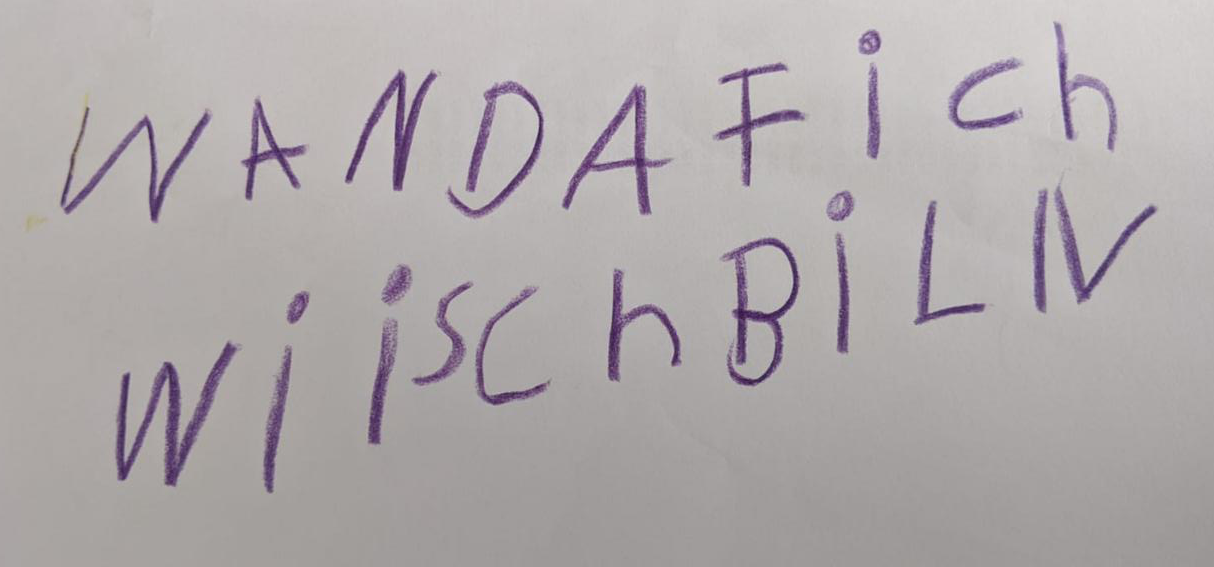
\includegraphics[width=0.9\textwidth]{graphics/wii}\\
  \Halbzeile
  \grau{\tiny Hannah aus Berlin mit 6 Jahren}
\end{frame}

\newcommand{\graphem}[1]{\ensuremath{\langle}#1\ensuremath{\rangle}}

\begin{frame}
  {Von welchen Schreibprinzipien weicht Hannah ab?}
  \centering 
  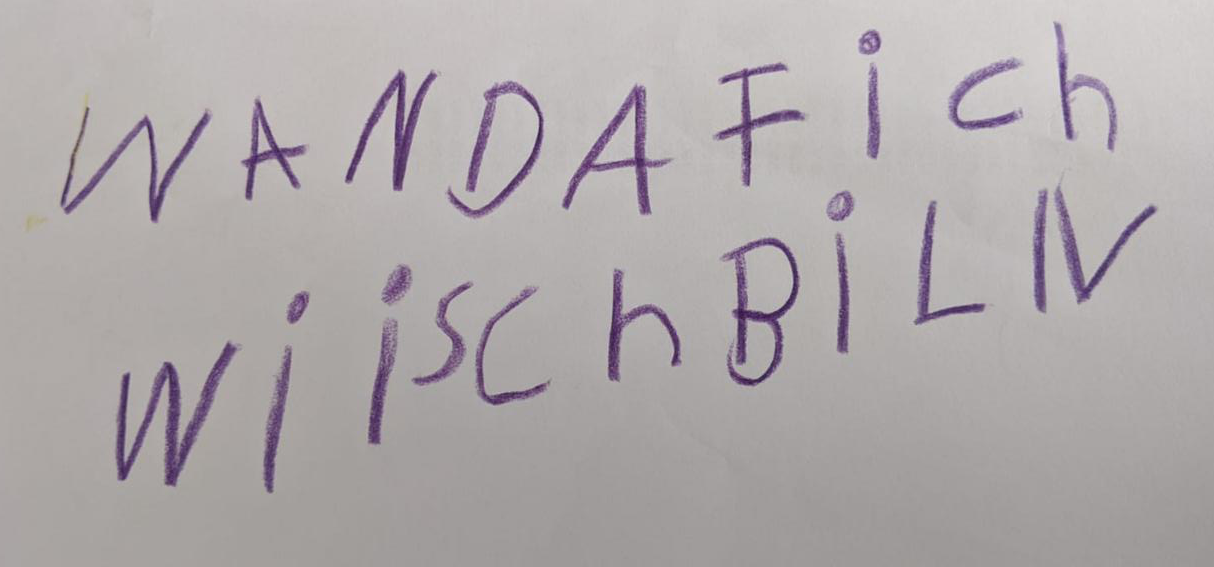
\includegraphics[width=0.2\textwidth]{graphics/wii}\\
  \Halbzeile
  \raggedright
  \begin{itemize}[<+->]
    \item Prinzipien der \alert{Majuskelschreibung} nicht gelernt
    \item Prinzip der \alert{Spatienschreibung} nicht gelernt
    \item \alert{\graphem{WAN}} | \alert{keine} Prinzipverletzung
    \item \alert{\graphem{DAF}} | \alert{phonetische} Abweichung vom Standard
    \item \alert{\graphem{ich}} | einwandfrei
    \item \alert{\graphem{Wii}} | \graphem{ii}-Dehnungsschreibung atypisch, \alert{Produktname}
    \item \graphem{\alert{sch}BiLN} | \alert{Abweichung von Prinzip} (Segmentschreibung) nicht gelernt
    \item \graphem{sch\alert{B}iLN} | \alert{phonetisch-phonologisches} "`Problem"'
    \item \graphem{schB\alert{i}LN} | \graphem{ie}-typische Dehnungsschreibung nicht gelernt
    \item \graphem{schBiL\alert{N}} | \alert{phonetische} Abweichung vom Standard
  \end{itemize}
\end{frame}

\begin{frame}
  {Warum kann die Schülerin nichts dafür?}
  \begin{itemize}[<+->]
    \item \alert{Hinhörschreibung} | Wir schreiben nicht, wie wir sprechen!\\
      "`Hinhören"' kann Hannah sehr gut.
      \Zeile
    \item \alert{Ausprobierschreibung} | \alert{Abweichungen von den Prinzipien}\\
      werden nicht beherrscht. Das ist das Ergebnis des Ausprobierens.
    \item Was wir uns selber erarbeiten (= ausprobieren),\\
      merken wir uns besonders gut.
      \Zeile
    \item Harte Prinzipien wurden nicht unterrichtet (Spatien, Majuskeln).
  \end{itemize}
\end{frame}

\section{Semesterplan}

\begin{frame}
  {Der ungefähre Semesterplan}
  \begin{enumerate}[<+->]
    \item 
    \item Wiederholung | segmentale Phonetik des Deutschen
    \item Wiederholung | segmentale Phonologie des Deutschen
    \item Segmentschreibungen (Buchstaben)
    \item Wortschreibungen
    \item syntaktische Schreibungen
    \item Interpunktion
    \item Gebrauchsschreibungen als Indikatoren für Prinzipien
  \end{enumerate}
\end{frame}


  
\fi

\makeatletter
\setcounter{lastpagemainpart}{\the\c@framenumber}
\makeatother

\appendix

\begin{frame}[allowframebreaks]
  {Literatur}
  \renewcommand*{\bibfont}{\footnotesize}
  \setbeamertemplate{bibliography item}{}
  \printbibliography
\end{frame}

\begin{frame}
  {Autor}
  \begin{block}{Kontakt}
    Prof.\ Dr.\ Roland Schäfer\\
    Institut für Germanistische Sprachwissenschaft\\
    Friedrich-Schiller-Universität Jena\\
    Fürstengraben 30\\
    07743 Jena\\[\baselineskip]
    \url{https://rolandschaefer.net}\\
    \texttt{roland.schaefer@uni-jena.de}
  \end{block}
\end{frame}

\begin{frame}
  {Lizenz}
  \begin{block}{Creative Commons BY-SA-3.0-DE}
    Dieses Werk ist unter einer Creative Commons Lizenz vom Typ \textit{Namensnennung - Weitergabe unter gleichen Bedingungen 3.0 Deutschland} zugänglich.
    Um eine Kopie dieser Lizenz einzusehen, konsultieren Sie \url{http://creativecommons.org/licenses/by-sa/3.0/de/} oder wenden Sie sich brieflich an Creative Commons, Postfach 1866, Mountain View, California, 94042, USA.
  \end{block}
\end{frame}

\mode<beamer>{\setcounter{framenumber}{\thelastpagemainpart}}

\end{document}
